%---------------------------------------------
% YaRrr! The Pirate's Guide to R
% Written by Nathaniel Phillips
% nathaniel.d.phillips.is@gmail.com
%---------------------------------------------

%----------------------------------------------------------------------------------------
%  Load packages and define custom functions
%----------------------------------------------------------------------------------------

\documentclass{tufte-book}\usepackage[]{graphicx}\usepackage[]{color}
%% maxwidth is the original width if it is less than linewidth
%% otherwise use linewidth (to make sure the graphics do not exceed the margin)
\makeatletter
\def\maxwidth{ %
  \ifdim\Gin@nat@width>\linewidth
    \linewidth
  \else
    \Gin@nat@width
  \fi
}
\makeatother

\definecolor{fgcolor}{rgb}{0.345, 0.345, 0.345}
\newcommand{\hlnum}[1]{\textcolor[rgb]{0.686,0.059,0.569}{#1}}%
\newcommand{\hlstr}[1]{\textcolor[rgb]{0.192,0.494,0.8}{#1}}%
\newcommand{\hlcom}[1]{\textcolor[rgb]{0.678,0.584,0.686}{\textit{#1}}}%
\newcommand{\hlopt}[1]{\textcolor[rgb]{0,0,0}{#1}}%
\newcommand{\hlstd}[1]{\textcolor[rgb]{0.345,0.345,0.345}{#1}}%
\newcommand{\hlkwa}[1]{\textcolor[rgb]{0.161,0.373,0.58}{\textbf{#1}}}%
\newcommand{\hlkwb}[1]{\textcolor[rgb]{0.69,0.353,0.396}{#1}}%
\newcommand{\hlkwc}[1]{\textcolor[rgb]{0.333,0.667,0.333}{#1}}%
\newcommand{\hlkwd}[1]{\textcolor[rgb]{0.737,0.353,0.396}{\textbf{#1}}}%

\usepackage{framed}
\makeatletter
\newenvironment{kframe}{%
 \def\at@end@of@kframe{}%
 \ifinner\ifhmode%
  \def\at@end@of@kframe{\end{minipage}}%
  \begin{minipage}{\columnwidth}%
 \fi\fi%
 \def\FrameCommand##1{\hskip\@totalleftmargin \hskip-\fboxsep
 \colorbox{shadecolor}{##1}\hskip-\fboxsep
     % There is no \\@totalrightmargin, so:
     \hskip-\linewidth \hskip-\@totalleftmargin \hskip\columnwidth}%
 \MakeFramed {\advance\hsize-\width
   \@totalleftmargin\z@ \linewidth\hsize
   \@setminipage}}%
 {\par\unskip\endMakeFramed%
 \at@end@of@kframe}
\makeatother

\definecolor{shadecolor}{rgb}{.97, .97, .97}
\definecolor{messagecolor}{rgb}{0, 0, 0}
\definecolor{warningcolor}{rgb}{1, 0, 1}
\definecolor{errorcolor}{rgb}{1, 0, 0}
\newenvironment{knitrout}{}{} % an empty environment to be redefined in TeX

\usepackage{alltt} % Use the tufte-book class which in turn uses the tufte-common class

\usepackage{microtype} % Improves character and word spacing
\usepackage{amsmath}
\usepackage{hyperref}
\usepackage{booktabs} % Better horizontal rules in tables
\usepackage[tikz]{bclogo}
\usepackage{listings}
%\usepackage{Sweave}
%\usepackage[demo]{graphicx}
\usepackage{fontspec}
\usepackage{caption}
\usepackage{subcaption}
\usepackage{listings}
\usepackage{color}
\usepackage{inconsolata}
\usepackage{float}
\usepackage{makeidx} % Used to generate the index

\usepackage{graphicx} % Needed to insert images into the document 

\graphicspath{{graphics/}} % Sets the default location of pictures
\setkeys{Gin}{width=\linewidth,totalheight=\textheight,keepaspectratio} % Improves figure scaling
\usepackage{fancyvrb} % Allows customization of verbatim environments
\fvset{fontsize=\normalsize} % The font size of all verbatim text can be changed here

\newcommand{\hangp}[1]{\makebox[0pt][r]{(}#1\makebox[0pt][l]{)}} % New command to create parentheses around text in tables which take up no horizontal space - this improves column spacing
\newcommand{\hangstar}{\makebox[0pt][l]{*}} % New command to create asterisks in tables which take up no horizontal space - this improves column spacing

\usepackage{xspace} % Used for printing a trailing space better than using a tilde (~) using the \xspace command
\newcommand{\blankpage}{\newpage\hbox{}\thispagestyle{empty}\newpage} % Command to insert a blank page

\newcommand{\newfun}[1]{\begin{LARGE} \begin{center} \texttt{#1} \end{center} \end{LARGE}}
\setcounter{tocdepth}{1}
\makeindex % Generate the index which is printed at the end of the document

\definecolor{mygreen}{rgb}{0,0.6,0}
\definecolor{mygray}{rgb}{0.5,0.5,0.5}
\definecolor{mymauve}{rgb}{0.58,0,0.82}
\usepackage{courier}



% 
% 
% <<setup, echo=FALSE>>=
% knit_hooks$set(source = function(x, options) {
%     paste("\\begin{lstset}{numbers=left, firstnumber=last}\n", x, 
%         "\\end{lstset}\n", sep = "")
% })
% @
% 



% 
% 
% \lstset{breaklines=true,showstringspaces=false}
% <<setup, include=FALSE, cache=FALSE>>=
% opts_chunk$set(fig.path = 'figure/listings-')
% options(replace.assign = TRUE, width=60)
% render_listings()
% @
% 


% 
% <<setup, echo=FALSE, eval = F>>=
% library(knitr)
% knit_hooks$set(source = function(x, options) {
%     paste("\\begin{lstlisting}[
%           numbers=left, 
%           firstnumber=last,
%           language=R,
%           stepnumber=1,
%           keywordstyle=\color{blue}
%           ]\n", x, 
%          "\\end{lstlisting}\n", sep = "")
%  })
%  @
%  
% % 
% 


% 
% \lstdefinestyle{ % 
%   language=R,                % the language of the code 
%   basicstyle=\footnotesize,           % the size of the fonts that are used for the code 
%   numbers=left,                   % where to put the line-numbers 
%   numberstyle=\tiny\color{gray},  % the style that is used for the line-numbers 
%   stepnumber=1,                   % the step between two line-numbers. If it's 1, each linwill be numbered 
%   numbersep=5pt,                  % how far the line-numbers are from the code 
%   backgroundcolor=\color{white},      % choose the background color. You must add \usepackage{color} 
%   showspaces=false,               % show spaces adding particular underscores 
%   showstringspaces=false,         % underline spaces within strings 
%   showtabs=false,                 % show tabs within strings adding particular underscores 
%   frame=single,                   % adds a frame around the code 
%   rulecolor=\color{black},        % if not set, the frame-color may be changed on line-breaks within not-black text (e.g. commens (green here)) 
%   tabsize=2,                      % sets default tabsize to 2 spaces 
%   captionpos=b,                   % sets the caption-position to bottom 
%   breaklines=true,                % sets automatic line breaking 
%   breakatwhitespace=false,        % sets if automatic breaks should only happen at whitespace also try caption instead of title 
%   keywordstyle=\color{blue},          % keyword style 
%   commentstyle=\color{dkgreen},       % comment style 
%   stringstyle=\color{mauve},         % string literal style 
%   escapeinside={\%*}{*)},            % if you want to add a comment within your code 
%   morekeywords={*,...}               % if you want to add more keywords to the set 
% } 


%----------------------------------------------------------------------------------------
%	BOOK META-INFORMATION
%----------------------------------------------------------------------------------------

\title{YaRrr! The Pirate's Guide to R}

\author{Dr. Nathaniel D. Phillips}

%\publisher{Publisher Name}

%----------------------------------------------------------------------------------------
\IfFileExists{upquote.sty}{\usepackage{upquote}}{}
\begin{document}




%----------------------------------------------------------------------------------------
%	INTRODUCTION
%----------------------------------------------------------------------------------------

%\cleardoublepage

\chapter{Introduction} % The asterisk leaves out this chapter from the table of contents


\begin{knitrout}
\definecolor{shadecolor}{rgb}{0.969, 0.969, 0.969}\color{fgcolor}\begin{kframe}
\begin{lstlisting}[numbers=left, 
          basicstyle=\footnotesize\ttfamily\linespread{0.01}\listingsfont,
          firstnumber=last, 
          numbersep=10pt, 
          showspaces=false,
          language=R,
          numberstyle=\color{mygray}, 
          keywordstyle=\color{blue},
          breaklines=false,
          aboveskip={0pt},
          belowskip={0pt},
          showstringspaces=false,
          breakatwhitespace=false,
          commentstyle=\color{purple!40!black},
          stringstyle=\color{orange}]
1 + 4\end{lstlisting}
\begin{verbatim}
## [1] 5
\end{verbatim}
\begin{lstlisting}[numbers=left, 
          basicstyle=\footnotesize\ttfamily\linespread{0.01}\listingsfont,
          firstnumber=last, 
          numbersep=10pt, 
          showspaces=false,
          language=R,
          numberstyle=\color{mygray}, 
          keywordstyle=\color{blue},
          breaklines=false,
          aboveskip={0pt},
          belowskip={0pt},
          showstringspaces=false,
          breakatwhitespace=false,
          commentstyle=\color{purple!40!black},
          stringstyle=\color{orange}]
5 - 9\end{lstlisting}
\begin{verbatim}
## [1] -4
\end{verbatim}
\begin{lstlisting}[numbers=left, 
          basicstyle=\footnotesize\ttfamily\linespread{0.01}\listingsfont,
          firstnumber=last, 
          numbersep=10pt, 
          showspaces=false,
          language=R,
          numberstyle=\color{mygray}, 
          keywordstyle=\color{blue},
          breaklines=false,
          aboveskip={0pt},
          belowskip={0pt},
          showstringspaces=false,
          breakatwhitespace=false,
          commentstyle=\color{purple!40!black},
          stringstyle=\color{orange}]
string <- "I am a string"\end{lstlisting}
\begin{lstlisting}[numbers=left, 
          basicstyle=\footnotesize\ttfamily\linespread{0.01}\listingsfont,
          firstnumber=last, 
          numbersep=10pt, 
          showspaces=false,
          language=R,
          numberstyle=\color{mygray}, 
          keywordstyle=\color{blue},
          breaklines=false,
          aboveskip={0pt},
          belowskip={0pt},
          showstringspaces=false,
          breakatwhitespace=false,
          commentstyle=\color{purple!40!black},
          stringstyle=\color{orange}]
a <- rnorm(100, mean = 1, sd = 2)\end{lstlisting}
\begin{lstlisting}[numbers=left, 
          basicstyle=\footnotesize\ttfamily\linespread{0.01}\listingsfont,
          firstnumber=last, 
          numbersep=10pt, 
          showspaces=false,
          language=R,
          numberstyle=\color{mygray}, 
          keywordstyle=\color{blue},
          breaklines=false,
          aboveskip={0pt},
          belowskip={0pt},
          showstringspaces=false,
          breakatwhitespace=false,
          commentstyle=\color{purple!40!black},
          stringstyle=\color{orange}]
# Load beanplot\end{lstlisting}
\begin{lstlisting}[numbers=left, 
          basicstyle=\footnotesize\ttfamily\linespread{0.01}\listingsfont,
          firstnumber=last, 
          numbersep=10pt, 
          showspaces=false,
          language=R,
          numberstyle=\color{mygray}, 
          keywordstyle=\color{blue},
          breaklines=false,
          aboveskip={0pt},
          belowskip={0pt},
          showstringspaces=false,
          breakatwhitespace=false,
          commentstyle=\color{purple!40!black},
          stringstyle=\color{orange}]
library(beanplot)\end{lstlisting}
\begin{lstlisting}[numbers=left, 
          basicstyle=\footnotesize\ttfamily\linespread{0.01}\listingsfont,
          firstnumber=last, 
          numbersep=10pt, 
          showspaces=false,
          language=R,
          numberstyle=\color{mygray}, 
          keywordstyle=\color{blue},
          breaklines=false,
          aboveskip={0pt},
          belowskip={0pt},
          showstringspaces=false,
          breakatwhitespace=false,
          commentstyle=\color{purple!40!black},
          stringstyle=\color{orange}]
beanplot(a)\end{lstlisting}
\end{kframe}
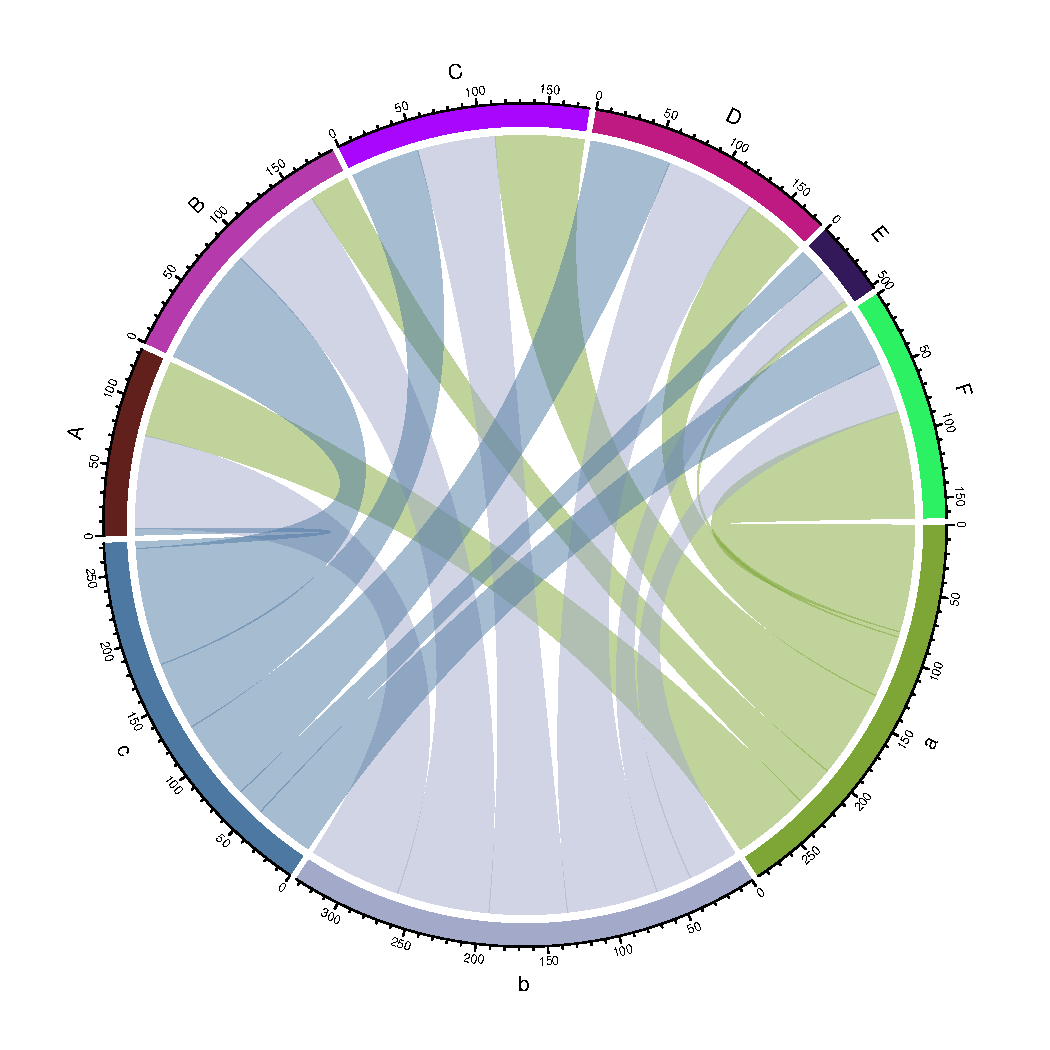
\includegraphics[width=\maxwidth]{figure/unnamed-chunk-1-1} 

\end{knitrout}


\begin{knitrout}
\definecolor{shadecolor}{rgb}{0.969, 0.969, 0.969}\color{fgcolor}\begin{kframe}
\begin{lstlisting}[numbers=left, 
          basicstyle=\footnotesize\ttfamily\linespread{0.01}\listingsfont,
          firstnumber=last, 
          numbersep=10pt, 
          showspaces=false,
          language=R,
          numberstyle=\color{mygray}, 
          keywordstyle=\color{blue},
          breaklines=false,
          aboveskip={0pt},
          belowskip={0pt},
          showstringspaces=false,
          breakatwhitespace=false,
          commentstyle=\color{purple!40!black},
          stringstyle=\color{orange}]
# Here is a second chunk\end{lstlisting}
\begin{lstlisting}[numbers=left, 
          basicstyle=\footnotesize\ttfamily\linespread{0.01}\listingsfont,
          firstnumber=last, 
          numbersep=10pt, 
          showspaces=false,
          language=R,
          numberstyle=\color{mygray}, 
          keywordstyle=\color{blue},
          breaklines=false,
          aboveskip={0pt},
          belowskip={0pt},
          showstringspaces=false,
          breakatwhitespace=false,
          commentstyle=\color{purple!40!black},
          stringstyle=\color{orange}]
rnorm(10)\end{lstlisting}
\begin{verbatim}
##  [1] -0.82879724 -0.16588616  1.88241393  0.04003067 -0.16041696
##  [6]  1.02417278 -0.66880172 -0.78739480 -1.97035410 -0.32198761
\end{verbatim}
\end{kframe}
\end{knitrout}


\backmatter

%----------------------------------------------------------------------------------------
%  BIBLIOGRAPHY
%----------------------------------------------------------------------------------------

\bibliography{bibliography} % Use the bibliography.bib file for the bibliography
\bibliographystyle{plainnat} % Use the plainnat style of referencing

%----------------------------------------------------------------------------------------

\printindex % Print the index at the very end of the document

\end{document}
